\chapterwithsubtitle{Tâche 5}{Comparer les meilleures solutions obtenues (optimum et temps de résolution) avec les heuristiques, par rapport à celle trouvées avec la relaxation choisie}
\vspace*{1.2cm}


\section{Convergence d'evolve-and-fix (tâche 2)}

Comme expliqué dans la partie portant sur la tâche 2 du projet, 
l'heuristique proposée fonctionne principalement sur des instances de très petite
taille et nécessite de fixer les variables de manière plus stratégique afin
d'éviter de violer les contraintes liées aux démarrages des générateurs
(de type 3.32 entre autres).

\begin{figure}[h!]
\begin{center}
	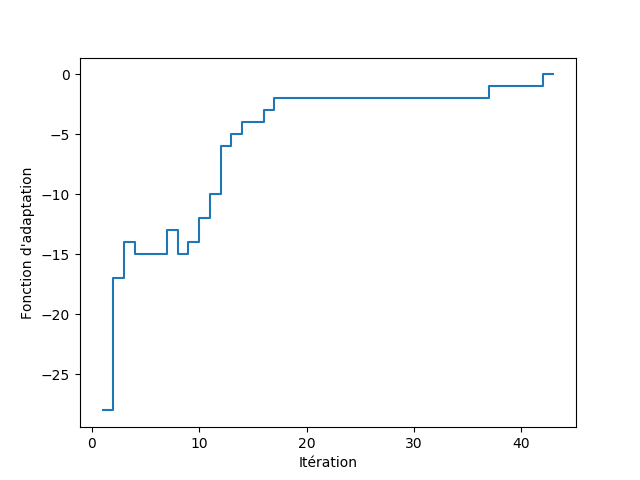
\includegraphics[width=.5\textwidth]{imgs/round}
	\caption{\'Evolution de la fonction d'adaptation calculée par evolve-and-fix
    sur l'instance \textit{inst-10-6-5-0.txt} - Méthode d'arrondi de la solution
    obtenue par la relaxation linéaire: Pour cette l'instance, le nombre de contraintes
    non satisfaites tombe rapidement à 0, permettant à l'heuristique de renvoyer
    une solution admissible.}
\end{center}
\end{figure}

Cependant, l'heuristique a l'avantage de ne posséder aucun paramètre si ce n'est ceux
de l'algorithme génétique, qui quant à eux peuvent être laissés à leurs valeurs par
défaut. En effet, les résultats obtenus sont fort robustes à l'ajustement des paramètres.
Les valeurs par défaut sont les suivantes:
\begin{itemize}
    \item Taille de la population: 100
    \item Nombre d'individus lors d'un tournoi: 2
    \item Taux de mutation: 2
    \item Nombre maximum d'itérations: 100000
\end{itemize}
\newpage
\section{Convergence du sous-gradient (tâches 3 et 4)}

Il est important de noter qu'evolve-and-fix trouve une solution plus aisément lorsqu'appliqué
à une solution proche de la zone admissible, en particuler la somme ergodique d'une (de préférence
longue) série de solutions primales non-faisables.

\begin{figure}[h!]
\begin{center}
    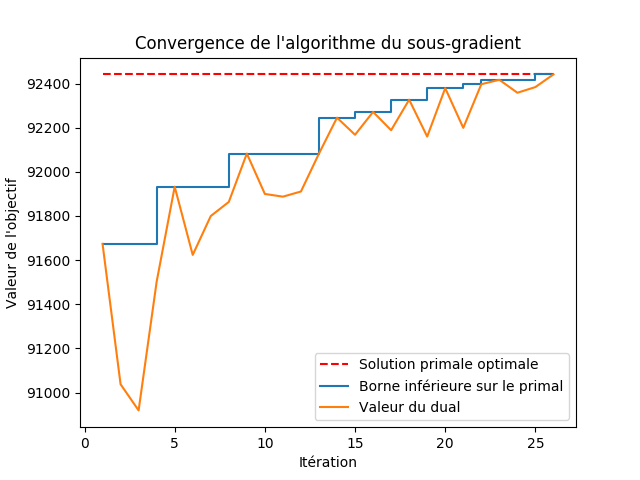
\includegraphics[width=.5\textwidth]{imgs/subgradient}
    \caption{Convergence du sous-gradient pour l'instance \textit{inst-10-6-5-0.txt}:
    Pour cette instance, la solution optimale du primal a été retrouvée.}
\end{center}
\end{figure}

Sur les plus petites instances fournies, le temps requis pour trouver la solution optimale du problème
d'origine (sans relaxation ni heuristique) est largement inférieur à celui pris par le sous-gradient
pour converger et trouver la solution optimale. Ce phénomène s'estompt rapidement lorsque la taille
du problème augmente (que ce soit par son nombre de scénarios, son nombre de générateurs ou son nombre
de périodes de temps). Il y a donc intérêt à utiliser la décomposition lagrangienne lorsque le problème
gagne en difficulté. De plus, les temps que nous avons mesuré ne tiennent pas compte de la nature
parallèle de la décomposition.

En effet nous avons fait le choix de \textbf{ne pas simuler la distribution de l'algorithme du sous-gradient}
car PuLP ne gère pas le parallélisme et est sujet à de nombreux bugs lorsqu'il est confronté au multiprocessing
sur une seule machine. Le gain potentiel de vitesse qu'il reste possible d'obtenir est considérable et est
d'au plus le nombre de scénarios du problème.

\section{Résultats}

Les deux tableaux qui suivent reprennent les solutions trouvées avec les différentes méthodes,
ainsi que les temps d'exécution. \textit{RL} fait référence à la relaxation linéaire:
la valeur de l'objectif correspondant n'est donc pas celui du problème d'origine mais de la
relaxation elle-même et est donc inférieure à la solution optimale.
Les solutions optimales des problèmes d'origine n'ont pas été reprises dans les résultats car, bien
que très rapides à calculer pour les plus petites instances, elles peuvent prendre un temps
démentiel sur certaines des instances utilisées.

\textit{$\lambda$RL} fait référence à la relaxation lagrangienne: la valeur de l'objectif est donc
celui de la solution primale obtenue de manière heuristique sur base de la dernière itération
de la méthode du sous-gradient. La colonne \textit{dual} donne à titre indicatif la dernière valeur obtenue
pour le dual lagrangien. Notons qu'il ne s'agit pas de la borne inférieure du primal et donc pas de la
meilleure valeur pour le dual. Comme il n'était malheureusement pas possible d'obtenir les résultats de toutes les instances dans un temps raisonnable avec l'approche de la décomposition lagrangienne, les résultats des instances non-traitées sont remplacés par le symbole "-". \textbf{Les valeurs sont indiquées en gras lorsque les solutions trouvées de manière heuristique sont optimales pour le primal}.

Les valeurs des paramètres utilisés dans l'algorithme de sous-gradient sont reprises à titre indicatif dans le tableau ci-dessous. Pour spécifier ces paramètres en ligne de commande, veuillez vous référer au début du rapport.
\begin{center}
\begin{tabular}{r|c|c|c|c|c|}
	& $\lambda$ & $\epsilon$ & $\alpha$ & $\rho$ & nar\\
	\hline \hline
	inst-10-6-5-x.txt & 0.01 & 0.01 & 2000 & 0.96 & 25 \\
	inst-10-6-10-x.txt & 0.01 & 0.01 & 5000 & 0.96 & 40 \\
	\hline	
\end{tabular}
\end{center}\newpage
\begin{landscape}

\begin{table*}[h!]\centering
\ra{1.3}
\begin{tabular}{@{}rrrcrrrcrrrr@{}}\toprule
& \multicolumn{2}{c}{RL} & \phantom{abc} & \multicolumn{3}{c}{Méthode d'arrondi} & \phantom{abc} & \multicolumn{4}{c}{$\lambda$RL}\\
\cmidrule{2-3} \cmidrule{5-7} \cmidrule{9-12}
& Objectif & Temps(s) & & Objectif & Temps(s) & Admissible & & Objectif & Temps(s) & Dual & Saut\\ \midrule

inst-10-6-5-0.txt & 91174.75 & 0.33 & & 94480.54 & 31.53 & - & & \textbf{92441.36} & 78.55 & \textbf{92441.36} & 0\% \\
inst-10-6-5-1.txt & 90652.18 & 0.30 & & 94580.37 & 30.45 & oui & & 94751.17 & 111.31 & 91886.78 & 3.02\% \\
inst-10-6-5-2.txt & 89810.63 & 0.28 & & 94891.98 & 5.42 & - & & - & - & - & - \\
inst-10-6-5-3.txt & 91470.78 & 0.34 & & 103855.17 & 30.70 & - & & \textbf{92685.26} & 56.85 & \textbf{92685.26} & 0\% \\
inst-10-6-5-4.txt & 91547.35 & 0.34 & & 101224.54 & 29.72 & - & & \textbf{92908.99} & 28.64 & \textbf{92908.99} & 0\% \\
inst-10-6-10-0.txt & 90751.45 & 0.76 & & 93219.45 & 17.31 & oui & & \textbf{91499.47} & 27.36 & \textbf{91499.47} & 0\% \\
inst-10-6-10-1.txt & 89549.23 & 0.68 & & 98493.06 & 48.37 & - & & \textbf{90476.24} & 174.04 & \textbf{90476.24} & 0\% \\
inst-10-6-10-2.txt & 90286.37 & 0.66 & & 95190.96 & 44.08 & oui & & \textbf{90934.95} & 164.12 & \textbf{90934.95} & 0\% \\
inst-10-6-10-3.txt & 91200.85 & 0.53 & & 95188.59 & 18.26 & oui & & \textbf{92549.49} & 62.70 & \textbf{92549.49} & 0\% \\
inst-10-6-10-4.txt & 90726.53 & 0.67 & & 94696.54 & 49.17 & - & & 94693.54 & 192.91 & 92131.74 & 2.71\% \\
inst-10-12-5-0.txt & 236718.61 & 0.69 & & 255901.57 & 37.68 & - & & - & - & - & - \\
inst-10-12-5-1.txt & 234103.99 & 0.74 & & 263560.52 & 27.64 & - & & - & - & - & - \\
inst-10-12-5-2.txt & 243033.56 & 0.82 & & 271783.36 & 42.32 & - & & - & - & - & - \\
inst-10-12-5-3.txt & 235307.27 & 0.79 & & 263751.59 & 38.17 & - & & - & - & - & - \\
inst-10-12-5-4.txt & 232639.77 & 0.85 & & 255517.90 & 23.88 & - & & - & - & - & - \\
inst-10-12-10-0.txt & 239023.59 & 1.31 & & 258728.97 & 70.95 & - & & - & - & - & - \\
inst-10-12-10-1.txt & 234931.20 & 1.69 & & 273970.32 & 96.84 & - & & - & - & - & - \\
inst-10-12-10-2.txt & 235774.17 & 1.49 & & 252770.10 & 90.19 & - & & - & - & - & - \\
inst-10-12-10-3.txt & 241277.17 & 1.43 & & 284073.02 & 80.20 & - & & - & - & - & - \\
inst-10-12-10-4.txt & 235551.55 & 1.84 & & 249891.31 & 93.06 & - & & - & - & - & - \\

\end{tabular}
\end{table*}
\end{landscape}
\newpage

\begin{landscape}

\begin{table*}[h!]\centering
\ra{1.3}
\begin{tabular}{@{}rrrcrrrcrrrr@{}}\toprule
& \multicolumn{2}{c}{RL} & \phantom{abc} & \multicolumn{3}{c}{Méthode d'arrondi} & \phantom{abc} & \multicolumn{4}{c}{$\lambda$RL}\\
\cmidrule{2-3} \cmidrule{5-7} \cmidrule{9-12}
& Objectif & Temps(s) & & Objectif & Temps(s) & Admissible & & Objectif & Temps(s) & Dual & Saut\\ \midrule

inst-10-24-5-0.txt & 478886.40 & 1.54 & & 544541.99 & 72.62 & - & & - & - & - & - \\
inst-10-24-5-1.txt & 475638.19 & 1.44 & & 557913.85 & 111.23 & - & & - & - & - & - \\
inst-10-24-5-2.txt & 469943.06 & 1.38 & & 526371.57 & 95.51 & - & & - & - & - & - \\
inst-10-24-5-3.txt & 473632.74 & 1.63 & & 506284.01 & 101.82 & - & & - & - & - & - \\
inst-10-24-5-4.txt & 476237.22 & 1.60 & & 510716.24 & 79.76 & - & & - & - & - & - \\
inst-10-24-10-0.txt & 490417.15 & 3.41 & & 576754.35 & 164.86 & - & & - & - & - & - \\
inst-10-24-10-1.txt & 477188.42 & 3.27 & & 536734.65 & 183.04 & - & & - & - & - & - \\
inst-10-24-10-2.txt & 475276.39 & 4.07 & & 554725.74 & 227.55 & - & & - & - & - & - \\
inst-10-24-10-3.txt & 482149.53 & 4.24 & & 545631.74 & 236.90 & - & & - & - & - & - \\
inst-10-24-10-4.txt & 475704.60 & 3.99 & & 539894.73 & 239.95 & - & & - & - & - & - \\

\end{tabular}
\end{table*}

\end{landscape}